\documentclass[journal,12pt,twocolumn]{IEEEtran}
\usepackage{amsthm}
\usepackage{graphicx}
\usepackage{mathrsfs}
\usepackage{txfonts}
\usepackage{stfloats}
\usepackage{pgfplots}
\usepackage{cite}
\usepackage{cases}
\usepackage{mathtools}
\usepackage{caption}
\usepackage{enumerate}	
\usepackage{enumitem}
\usepackage{amsmath}
\usepackage[utf8]{inputenc}
\usepackage[english]{babel}
\usepackage{multicol}
%\usepackage{xtab}
\usepackage{longtable}
\usepackage{multirow}
%\usepackage{algorithm}
%\usepackage{algpseudocode}
\usepackage{enumitem}
\usepackage{mathtools}
\usepackage{gensymb}
\usepackage{hyperref}
%\usepackage[framemethod=tikz]{mdframed}
\usepackage{listings}
    %\usepackage[latin1]{inputenc}                                 %%
    \usepackage{color}                                            %%
    \usepackage{array}                                            %%
    \usepackage{longtable}                                        %%
    \usepackage{calc}                                             %%
    \usepackage{multirow}                                         %%
    \usepackage{hhline}                                           %%
    \usepackage{ifthen}                                         %%
  \providecommand{\nCr}[2]{\,^{#1}C_{#2}}
  \providecommand{\nPr}[2]{\,^{#1}P_{#2}}
  \lstset{
%language=C,
frame=single, 
breaklines=true,
columns=fullflexible
}

\title{Assignment 4
\\Probability and Random Variables }
\author{Swati Mohanty (EE20RESCH11007) }
\date{February 2021}

\begin{document}

\maketitle


\section{Problem}
Find the probability distribution of
\\(i) number of heads in two tosses of a coin.
\\(ii) number of tails in the simultaneous tosses
of three coins.
\\(iii) number of heads in four tosses of a coin.

\section{Solution}

(i)Let the event be defined as
\\X = Number of heads when a coin is tossed twice
\\Outcomes =\{HH,HT,TH,TT\}
\\Hence the probability distribution of X is: 

\begin{center}
\begin{tabular}{ |c|c|c|c| } 
 \hline
 X & 0 & 1 & 2 \\\hline 
 P(X) & 1/4 & 1/2 & 1/2 \\ 
 \hline
\end{tabular}
\end{center}
(ii)Let the event be defined as
\\X = Number of tails in the simultaneous tosses of three coins.
\\Outcomes =\{ HHH,HHT,HTH,HTT,THH,THH,TTH,
TTT\}
\\Hence the probability distribution of X is: 

\begin{center}
\begin{tabular}{ |c|c|c|c|c| } 
 \hline
 X & 0 & 1 & 2 & 3 \\ \hline
 P(X) & 1/8 & 3/8 & 3/8 & 1/8 \\ 
 \hline
\end{tabular}
\end{center}
(iii)Let the event be defined as
\\X = Number of heads in four tosses of a coin.
\\Outcomes =\{ HHHH,HHHT,HHTH,HHTT,HTHH,
HTHH,HTTH,HTTT,THHH,THHT,THTH,THTT,
TTHH, TTHH,TTTH,TTTT\}
\\Hence the probability distribution of X is: 

\begin{center}
\begin{tabular}{ |c|c|c|c|c|c| } 
 \hline
 X & 0 & 1 & 2 & 3 & 4 \\ \hline
 P(X) & 1/16 & 1/4 & 3/8 & 1/4 & 1/16 \\ 
 \hline
\end{tabular}
\end{center}
\\The PDF graphs were plotted using the python code.
\begin{figure}[h]
\renewcommand{\theenumi}{1}
\centering
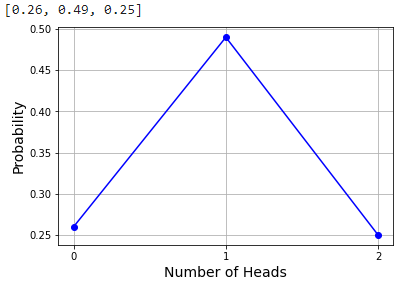
\includegraphics[ width=\columnwidth , height =4cm]{2toss_coin.PNG}
\caption{PDF for tossing a fair coin twice }
\label{Fig:1}
\\
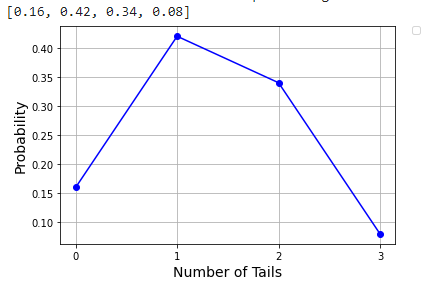
\includegraphics[ width=\columnwidth , height =5cm]{3toss_coin.PNG}
\caption{PDF for tossing a fair coin thrice }
\label{Fig:2}\\
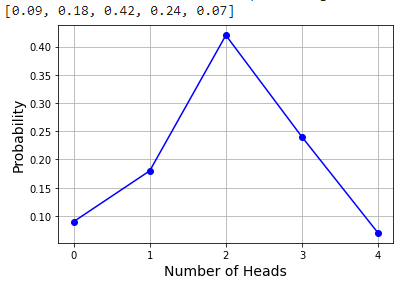
\includegraphics[ width=\columnwidth , height =5cm]{4toss_coin.PNG}
\caption{PDF for tossing a fair coin 4 times }
\label{Fig:3}
\end{figure}


\\\textbf{Download python code from here}\\
\begin{lstlisting}
https://github.com/Swati-Mohanty/AI5002/blob/main/Assignment_4/codes/cointoss.py
\end{lstlisting}
\\\textbf{Download latex code from here-}\\
\begin{lstlisting}
https://github.com/Swati-Mohanty/AI5002/blob/main/Assignment_4/codes/assignment4.tex
\end{lstlisting}

\end{document}
